

\documentclass[OPS,authoryear,toc]{lsstdoc}
% lsstdoc documentation: https://lsst-texmf.lsst.io/lsstdoc.html

% Package imports go here.

\usepackage[nonumberlist,nogroupskip,toc,numberedsection=autolabel,style=index]{glossaries}
\usepackage{environ}
\usepackage{enumitem}

% Local commands go here.

% DO NOT EDIT - generated by /Users/womullan/LSSTgit/lsst-texmf/bin/generateAcronyms.py from https://lsst-texmf.lsst.io/.
\newacronym {AD} {AD} {Associate Director}
\newacronym {AMCL} {AMCL} {Aura Management Council for LSST}
\newacronym {AP} {AP} {Alert Production}
\newacronym {AWS} {AWS} {Amazon Web Services, one of the largest \gls{cloud} computing providers.}
\newacronym {CI} {CI} {\gls{cyberinfrastructure}}
\newacronym {DAQ} {DAQ} {Data Acquisition System}
\newacronym {DBB} {DBB} {Data Back Bone}
\newacronym {DM} {DM} {Data Management}
\newacronym {DMTN} {DMTN} {DM Technical Note}
\newacronym {DOE} {DOE} {Department Of Energy}
\newacronym {DRP} {DRP} {Data Release Production}
\newacronym {FTE} {FTE} {Full Time Equivalent}
\newacronym {ITC} {ITC} {Information Technology Center}
\newacronym {LDF} {LDF} {LSST Data Facility}
\newacronym {LSST} {LSST} {Large Synoptic Survey Telescope}
\newacronym {NCOA} {NCOA} {National Center for Optical-Infrared Astronomy}
\newacronym {NCSA} {NCSA} {National Center for Supercomputing Applications}
\newacronym {NSF} {NSF} {National Science Foundation}
\newacronym {OPS} {OPS} {Operations}
\newacronym {OPSTN} {OPSTN} {Operations Technical Note, document identifier handle}
\newacronym {QA} {QA} {Quality Assurance}
\newglossaryentry {Qserv} {name={Qserv}, description={Proprietary \gls{LSST} Database system}}
\newglossaryentry {S3} {name={S3}, description={Structured, imperative high level computer programming language, used as implementation language for the Virtual Machine Environment (\gls{VME}) operating system}}
\newacronym {SDQA} {SDQA} {Science Data Quality Assurance}
\newacronym {SLAC} {SLAC} {No longer an acronym; formerly Stanford Linear Accelerator Center}
\newacronym {SRE} {SRE} {Site Reliability Engineering}
\newacronym {US} {US} {United States}
\newacronym {VME} {VME} {Virtual Machine Environment}
\newglossaryentry {cloud} {name={cloud}, description={A visible mass of condensed water vapor floating in the atmosphere, typically high above the ground or in interstellar space acting as the birthplace for stars.  Also a way of computing (on other peoples computers leveraging their services and availability).}}
\newglossaryentry {cyberinfrastructure} {name={cyberinfrastructure}, description={Sometimes denoted \gls{CI}, A term first used by the \gls{US} National Science Foundation (\gls{NSF}), and it typically is used to refer to information technology systems that provide particularly powerful and advanced capabilities.}}
\newglossaryentry {software} {name={software}, description={The programs and other operating information used by a computer.}}

\makeglossaries

% To add a short-form title:
% \title[Short title]{Title}
\title{Alternative science operations approach for  \gls{LSST} }

% Optional subtitle
% \setDocSubtitle{A subtitle}

\author{%
William O'Mullane
}

\setDocRef{OPSTN-001}

\date{\today}

% Optional: name of the document's curator
% \setDocCurator{The Curator of this Document}

\setDocAbstract{%
After the Kavli workshop Petabytes to Science we have a suggested framework for data processing and disemination. This note cosiders how \gls{LSST} might fit in such a scheme.
}

% Change history defined here.
% Order: oldest first.
% Fields: VERSION, DATE, DESCRIPTION, OWNER NAME.
% See LPM-51 for version number policy.
\setDocChangeRecord{%
  \addtohist{1}{YYYY-MM-DD}{Unreleased.}{William O'Mullane}
}

\begin{document}

% Create the title page.
% Table of contents is added automatically with the "toc" class option.

\mkshorttitle
%switch to \maketitle if you wan the title page and toc


% ADD CONTENT HERE ... a file per section can be good for editing
\section{Introduction} \label{sec:intro}

We are currently experimenting with Google and Amazon services for science platform and processing.
These services are priced to deliver compute and storage - our current model at the LDF is also service oriented but
is not proceed in the same manner making comparisons difficult. It has been difficult to get an alternative cost model
together. An initial approach to a cloud costing was outlined in \citeds{DMTN-072}, this approach was to try to cost the hardware and compare to cloud pricing.

In this document a radical restructuring of LSST operations is explored - a technology stack underpinned by commodity services which could be provided by commercial providers or computing centers. Here we look first at how we would run something like this -we can then leave one free variable which is the cost of the underlying compute and storage services. This will both help to
sanity check the LDF costing and potentially allow us to have a ball park for assessing commodity provider offers.



\section{Plugable service oriented architecture} \label{sec:arc}

In the Kavli workshop in Vegas (Feb 2019 \cite{2019arXiv190505116B}) we took a long term view to astronomy archives and data processing.
We suggested a layered service model as depicted in \figref{fig:CI}\footnote{The full document is here \url{https://petabytestoscience.github.io/PetaBytes-2019-04-26.pdf}}.
Our requirements are no longer unique and we have access to a wealth of open source \gls{software}, commodity hardware, and managed \gls{cloud} services (offered by commercial providers and federally-funded institutions) that are well positioned to meet the needs of \gls{LSST} \cite{2019AAS...23345706M, 2019AAS...23324505B}.


\begin{figure}
    \centering
    \includegraphics[width=1.\textwidth]{images/CI-Layers}
    \caption{An example a \gls{cyberinfrastructure} built on an Infrastructure as Code design model. Note that while this example does not have astronomy-specific tooling, our recommendations highlight the importance of developing astro-specific layers that are fully accessible to scientists in both  the application  and the graphical interface layers. \label{fig:CI}}
\end{figure}


We took \figref{fig:CI} and made a more \gls{LSST} oriented version in \figref{fig:CI-LSST}. This is pretty close to how we are currently but we do not treat the compute and storage as pure services.

\begin{figure}
    \centering
    \includegraphics[width=1.\textwidth]{images/CI-LSST}
    \caption{An example \gls{LSST}  \gls{cyberinfrastructure} built analogous to the \gls{CI} model shown in \figref{fig:CI}.}
% Original https://docs.google.com/presentation/d/16w5WVe-_xNLXWudNKqJu9IEKGDQ8oIB0eDiqWP_SUnE/edit?usp=sharing
    \label{fig:CI-LSST}
\end{figure}\

In important part of following this architecture is the ability to choose best in class components. In the science platform for example we have probably the best notebook implementation but we could possibly pick up a better portal. In processing \gls{NCSA} insist on a shared noting approach - a move to an \gls{Object Storage} could profoundly change that. It may raise other questions though on replication and redundancy. Then the shared nothing approach brings its own problems for deployment and \gls{QA}.

A more service oriented approach should allow us to move between service providers to use the best in class for our underlying services as well.  A clear model, understood by many, will make \gls{QA} an easier task as well.


Getting to operations in this model will require some rethinking in construction - construction is a big ship which is already steaming ahead so a change in course will take some effort. It is absolutely worth pursuing though.






\section{Data Production Department }\label{sec:sciops} \label{sec:dataprod}

The role of data production within \gls{LSST} is to deliver \gls{LSST}'s science products: the science images, the alert stream, the annual data releases, the science \gls{software}, and the Science Platform. In the current ops proposal not all groups required to do this are under control of Science operations.

\figref{fig:opsorg} gives a view of the Data Production teams which combine some of the old science operations  and \gls{LDF} departments. This is far more analogous to Data Management moving into operations than in the current proposal and would make for a smoother transition.

\begin{figure}
\begin{center}
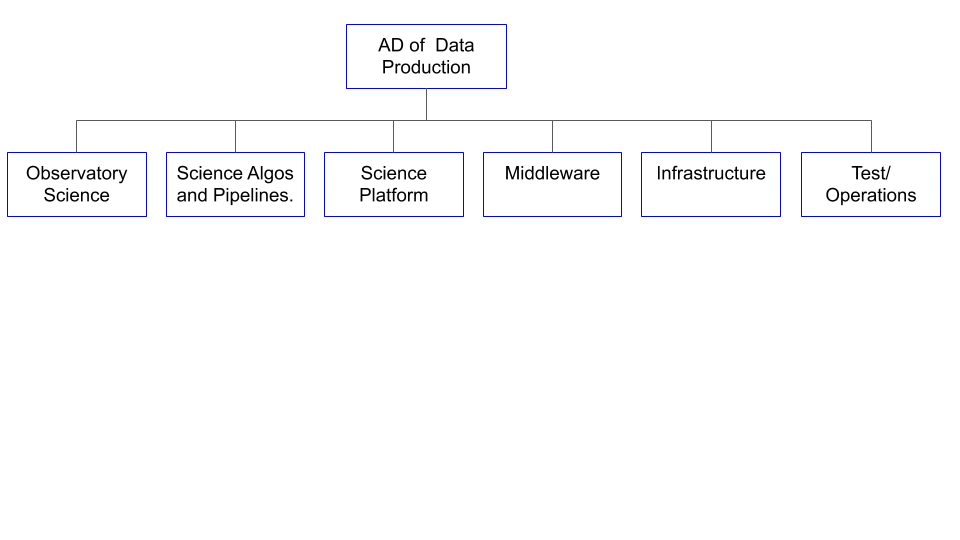
\includegraphics[width=0.9\textwidth,trim=0cm 10cm 0 0, clip]{figures/SciOpsOrg}
\caption{Possible configuration of Science Operations Department for operations of \gls{LSST} \label{fig:sciopsorg}}
\end{center}
% original https://docs.google.com/presentation/d/1wIN6Dj_rPn8TASBUkAm6_-Yh255Gz9VbwFi61t4LCFs/edit#slide=id.g55f7c0247e_0_2
\end{figure}

The \gls{FTE} counts are estimated in \tabref{tab:FTE}, which also gives the team sizes form the operations proposal for comparison.
A brief description of the teams is given in \secref{sec:teams}.
 \begin{longtable} { |p{0.3\textwidth}  |r  |r  |r  |r |} 
\caption{Size (in FTE) of the various teams in data production department with sizes including LDF teams from the proposal in the fourth column - a zero imples the team did not exist inthe proposal. \label{tab:FTE}}\\ 
\hline 
\textbf{Team}&\textbf{2023}&\textbf{2026}&\textbf{2023(P)}&\textbf{Note} \\ \hline
{Management (AD)}&{1.5}&{1.5}&{1}& \\ \hline
{Observatory Science }&{5.5}&{5.5}&{5.5}&{System performance?} \\ \hline
{Science Platform}&{6}&{6}&{6.5}& \\ \hline
{Science Algos and Pipelines}&{22}&{16}&{21}&{QA  to system performance?} \\ \hline
{Middleware}&{7.5}&{6.5}&{0}& \\ \hline
{Infrastructure}&{8}&{7}&{0}&{ } \\ \hline
{Verification/ Operations}&{5}&{4}&{0}& \\ \hline
{LDF Management (AD) }&{0}&{0}&{3}&{In infrastruture} \\ \hline
{LDF Scientific Prod. Services}&{0}&{0}&{6.75}&{In Verification/ operations} \\ \hline
{LDF ITC Security}&{0}&{0}&{8.5}&{Some in infrastructure/ middleware } \\ \hline
{LDF Prod. Services Soft.}&{0}&{0}&{7.6}&{Some in infrastructure} \\ \hline
{LDF ITC and Facilities}&{0}&{0}&{13}&{Should be in services charges} \\ \hline
\textbf{Total  FTE}&\textbf{55.5}&\textbf{46.5}&\textbf{72.85}& \\ \hline
\end{longtable}


\subsection{Teams }\label{sec:teams}
\figref{fig:sciopsorg} introduces several teams some of which were not in the original ops proposal. I  little detail is given here about each.

\subsubsection{Observatory Science}
As in the ops proposal the primary responsibility of this team is to understand the end-to-end impact of the Observatory hardware and environment on the science images and to work with the Observatory Operations department to ensure that the image quality meets requirements.

\textbf{This team may be better  in Observatory operations department }

\subsubsection{Science algorithms and pipelines}
This team is responsible to assess and assure the alert stream and annual data releases.
In the submitted proposal this includes extensive \gls{QA} to compare the data products against requirements -
this may be be better merged with Sytem Perfomance/Verification.
The main responsibility  of this team  would then be the  underlying \gls{software} pipelines themselves. Monitoring and updating the calibration plan and algorithmic implementation is also a responsibility of this team. The Calibration Support Scientist on the Observatory Science team will be responsible for monitoring the physical implementation of the calibration plan at the summit.
In \tabref{tab:FTE} this team is initially sized similarly to the AP/DRP teams in construction. There will be signifcant maintenance in the first two or three years of operations. As mentioned above there may be some consolidation with \gls{QA} activites in System Performance.

\subsubsection{Science platform  }
This team will be responsible for maintaining and evolving LSST’s user access portal, the Science Platform. This will include keeping up with evolving technologies and computing infrastructure, as well as providing basic code-base maintenance, bug fixes, and low-level response to science community and internal \gls{LSST} requests for new features.

\subsubsection{Middleware }
In a service oriented model with a layered architecture as outlined in \secref{sec:arc} it is essential to have a cross cutting team who compose and debug services.
Software such as the \texttt{butler}  is not part of the pipeline but the pipeline needs it. In house developments such as \gls{Qserv} should be covered here (1.5FTE has been included f0r this - DOE/SLAC personnel - could be 2).
This would also cover the builds and how the code interacts with the infrastructure (\secref{sec:infra}.

\subsubsection{Infrastructure, Site Reliability Engineering  } \label{ses:infra}
This is for deployment of of various systems and pipelines. Configuration is included in this. There needs to be a couple of people who manage keys/secrets
for access to commodity services. We would need a security resource as well as database expertise.  This then implies using tooling for system management as
provided by e.g. \gls{AWS} console.

In general an \gls{SRE} team is responsible for the availability, latency, performance, efficiency, change management, monitoring, emergency response and capacity planning of their services \cite{Beyer:2016:SRE:3006357}.

This team would include paying for a liaison at any service provider e.g. Google Professional Services or a Service Manager at \gls{NCSA}. (2FTE calculated)

\subsubsection{Verification/Operations }
This team will take and verify new releases for operations before they are deployed to the operations system. They will monitor the operational system to make sure it is functioning - they should have some science knowledge to know it is actually working properly as opposed to not just giving errors. A team of 4 should be able to handle this.
Some support for this is assumed from IN2P3 .







\section{Conclusion}\label{sec:conclusion}
 A restructuring of operations would  give more transparent cost, allow for a better comparison to commodity pricing for many services and would
yield considerable savings.



\appendix
% Include all the relevant bib files.
% https://lsst-texmf.lsst.io/lsstdoc.html#bibliographies
\section{References} \label{sec:bib}
\bibliography{lsst,lsst-dm,refs_ads,refs,books}

%Make sure lsst-texmf/bin/generateAcronyms.py is in your path
%section{Acronyms and glossary items}\label{sec:acronyms}
\printglossaries
%\addtocounter{table}{-1}
\begin{longtable}{|l|p{0.8\textwidth}|}\hline
\textbf{Acronym} & \textbf{Description}  \\\hline

AD & Associate Director \\\hline
AMCL & Aura Management Council for LSST \\\hline
AWS & Amazon Web Services, one of the largest cloud computing providers. \\\hline
CI & \gls{cyberinfrastructure} \\\hline
DAQ & Data Acquisition System \\\hline
DBB & Data Back Bone \\\hline
DM & Data Management \\\hline
DMTN & DM Technical Note \\\hline
DOE & Department Of Energy \\\hline
FTE & Full Time Equivalent \\\hline
ITC & Information Technology Center \\\hline
LDF & LSST Data Facility \\\hline
LSST & Large Synoptic Survey Telescope \\\hline
NCOA & National Center for Optical-Infrared Astronomy \\\hline
NCSA & National Center for Supercomputing Applications \\\hline
NSF & National Science Foundation \\\hline
OPS & Operations \\\hline
OPSTN & Operations Technical Note, document identifier handle \\\hline
QA & Quality Assurance \\\hline
Qserv & Proprietary LSST Database system \\\hline
S3 & Structured, imperative high level computer programming language, used as implementation language for the Virtual Machine Environment (\gls{VME}) operating system \\\hline
SDQA & Science Data Quality Assurance \\\hline
SLAC & No longer an acronym; formerly Stanford Linear Accelerator Center \\\hline
SRE & Site Reliability Engineering \\\hline
US & United States \\\hline
VME & Virtual Machine Environment \\\hline
cloud & A visible mass of condensed water vapor floating in the atmosphere, typically high above the ground or in interstellar space acting as the birthplace for stars.  Also a way of computing (on other peoples computers leveraging their services and availability). \\\hline
cyberinfrastructure & Sometimes denoted CI, A term first used by the US National Science Foundation (\gls{NSF}), and it typically is used to refer to information technology systems that provide particularly powerful and advanced capabilities. \\\hline
software & The programs and other operating information used by a computer. \\\hline
\end{longtable}

\end{document}
